\chapter{Time series}
\label{ch:time-series}

%\section{Tijdreeksen \& voorspellingen}
%
%\begin{definition}[Tijdsreeks]
%	Een tijdreeks is een opeenvolging van observaties van een willekeurige variabele in functie van de tijd.
%\end{definition}
%
%Een tijdreeks is dus eens stochastisch proces. Denk hierbij maar aan:
%\begin{itemize}
%	\item maandelijkse vraag naar melk
%	\item jaarlijkse instroom van studenten bij de Hogeschool
%	\item dagelijks debiet van een rivier
%\end{itemize}
%
%Het voorspellen van tijdreeksen is een belangrijk onderdeel van onderzoek omdat ze vaak de basis vormen voor beslissingsmodellen. Voorbeelden hiervan zijn :
%
%\begin{itemize}
%	\item algemene ontwikkeling van toekomstplannen (investeringen, capaciteit \dots)
%	\item plannen van budgettering om tekortkomingen te vermijden (operationeel budget, marketing budget \dots)
%	\item competitieve leveringstijden te bezorgen van een bedrijf
%	\item ondersteuning van financi\"ele objectieven
%	\item onzekerheid vermijden
%	\item de mogelijkheid om ontwikkelingen in de verkeersveiligheid
%kwantitatief te modelleren
%\end{itemize}
%
%Tijdreeksen modelleren is een statistisch probleem: we gaan ervan uit dat de observaties vari\"eren volgens een bepaalde kansdichtheidsfunctie in functie van de tijd. 
%
%Er zijn verschillende types modellen in gebruik voor het analyseren van tijdreeksen. Deze modellen hebben met elkaar gemeen dat ze in principe niet alleen de ontwikkeling in een geobserveerde tijdreeks kunnen beschrijven, maar dat we ze ook kunnen gebruiken om verklaringen voor de ontwikkeling in een geobserveerde tijdreeks te vinden, en om de toekomstige waarden van de
%ontwikkeling in een geobserveerde tijdreeks te voorspellen. Hun geschiktheid voor het verwezenlijken van deze doelstellingen loopt echter sterk uiteen. In dit hoofdstuk beperken we ons tot het gebruik van tijdreeksen met een geschiedenis om tijdsafhankelijke modellen te bepalen. 
%
%\section{Tijdreeksmodellen}
%\subsection{Wiskundig model}
%Ons doel is het opstellen van een model dat een verklaring vindt voor de geobserveerde data en dat toelaat om observaties in de toekomst zo goed mogelijk te voorspellen. Het simpelste model dat je kan bedenken is een model waarbij een constante $b$ gebruikt wordt met variaties rond $b$ bepaald door een willekeurige variabele $\epsilon_{t}$ zoals in vergelijking \ref{eq:constante}. 
%
%\begin{equation}
%	X_{t} = b + \epsilon_{t}
%\label{eq:constante}
%\end{equation}
%
%\begin{description}
%	\item [$X_{t}$] stelt een random variabele voor dat de onbekende is op tijdstip $t$.
%	\item [$x_{t}$] stelt een observatie voor op tijdstip $t$ (en is dus gekend). 
%	\item [$\epsilon_{t}$] noemt met de \textit{storing} (engels \textsl{noise}) en wordt geacht een gemiddelde van $0$ te hebben met variantie $\sigma^{2}$ en normaal verdeeld. 
%\end{description}
%
%\begin{figure}[htbp]
%	\centering
%		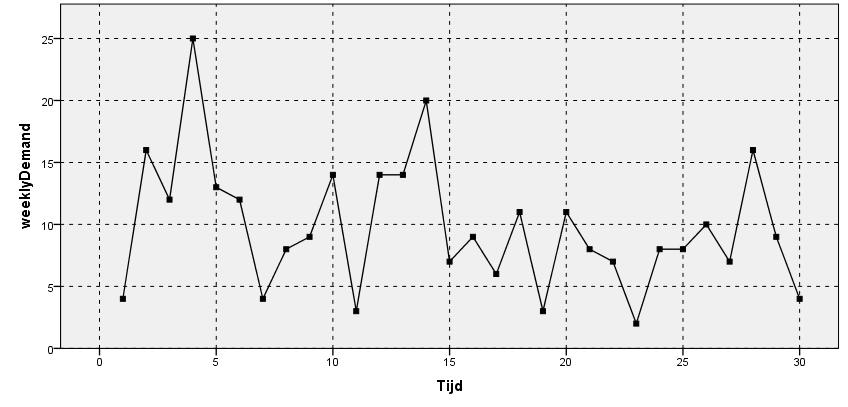
\includegraphics[width=\textwidth]{images/tijdsreeksen/tijdsreeks11.jpg}
%	\caption{Een tijdreeks voor een wekelijkse vraag voor een bepaald product}
%	\label{fig:tijdreeks11}
%\end{figure}
%
%
%We kunnen ook ervan uit gaan dat er een lineair verband is:
%
%\begin{equation}
%	X_{t} = b_{0} + b_{1} \times t + \epsilon_{t}
%\label{eq:lineair8}
%\end{equation}
%
%De vergelijking in \ref{eq:constante} en \ref{eq:lineair8} zijn speciale gevallen van het polynomiaal geval:
%
%\begin{equation}
%	X_{t} = b_{0} + b_{1} t + b_{2} t^{2} + \dots + b_{n} t^{n} + \epsilon_{t} 
%\label{eq:polynomiaal}
%\end{equation}
%
%\begin{exercise}
%	Wat zou volgende tijdreeks kunnen voorstellen?
%	\begin{equation}
%		X_{t} = b_{0} + b_{1} \sin(\frac{2\pi t}{4}) + b_{1} \cos(\frac{2\pi t}{4}) + \epsilon_{t}
%	\label{eq:seasonal}
%\end{equation}
%\end{exercise}
%
%Antwoord: dit is een cyclische tijdreeks met periode $= 4$. Dit zou bijvoorbeeld kunnen gebruikt worden bij een tijdreeks voor seizoenen.
%
%\subsubsection{Algemeen}
%
%In elk model beschouwd is de tijdreeks een functie van tijd en parameters van het model. We kunnen algemeen stellen dat:
%
%\begin{equation}
%	X_{t} = f(b_{0}, b_{1}, b_{2}, \dots , b_{t}, t) + \epsilon_{t}
%\label{eq:general}
%\end{equation}
%
%We aanvaarden vervolgens nog volgende stellingen:
%\begin{itemize}
%	\item Het model gaat uit van twee componenten van variabiliteit: het gemiddelde van de voorspellingen verandert met de tijd en de variaties tot dit gemiddelde vari\"eren willekeurig.
%	\item De residuen van het model ($X_{t} - x_{t}$) zijn homoscedastisch : dat wil zeggen in de tijd een constante variantie hebben.
%\end{itemize}
%
%Eenmaal het model gekozen, rest enkel nog het  probleem van het schatten van de parameters voor vergelijking \ref{eq:general}. Dit is wat in de volgende stukken besproken zal worden.
%
%\section{Schatten van de parameters}
%Eenmaal een model geselecteerd wordt, is het aan de onderzoeker om de parameters te gaan schatten, i.e. parameters die ervoor zorgen dat het model de geobserveerde waarden zo goed mogelijk benaderen. Meestal gaan we ervan uit dat alle waarden gelijkwaardig zijn, maar dat is niet zo bij tijdreeksen. Aangezien onze onafhankelijke parameter de tijd is moeten we methoden bekomen die ervoor zorgen dat recentere data belangrijker zijn dat oude data. 
%
%In wat volgt beschrijven we de tijdreeksen met geschatte waarden voor de parameters. We zetten hievoor een hoedje op de parameters:
%
%\[ \widehat{b}_{1}, \widehat{b}_{2} \dots \widehat{b}_{n} \] 
%
%Het schatten van de variatie voor $\sigma_{\epsilon}$ duiden we aan als $\widehat{\sigma}_{\epsilon}$.
%
%\subsection{Voorbeeld - moving average}
%
%\begin{table}[t]
%\centering
%    \begin{tabular}{|l|l|l|l|l|l|l|l|l|l|}
%    \hline
%    4 & 16 & 12 & 25 & 13 & 12 & 4 & 8  & 9 & 14 \\ \hline
%    3 & 14 & 14 & 20 & 7  & 9  & 6 & 11 & 3 & 11 \\ \hline
%    8 & 7  & 2  & 8  & 8  & 10 & 7 & 16 & 9 & 4  \\ \hline
%    \end{tabular}
%		\label{tab:data}
%		\caption{Voorbeeld data van vraag voor product, zie figuur \ref{fig:tijdreeks11}}
%\end{table}
%
%Stel dat de statisticus de data in tabel \ref{tab:data} tot het twintigste datapunt beschikbaar heeft (bekende data). De onderzoeker kent de datapunten vanaf het twintigste datapunt niet en moet deze gaan voorspellen. Een eerste model dat gebruikt zou kunnen worden is het constante model zoals in \ref{eq:constante}. 
%
%Met dit model, zijn de waarden random waarden uit een populatie met gemiddelde $b$. De beste schatter voor $b$ is het gemiddelde van deze twintig data punten. 
%
%\[ \widehat{b} = \frac{1}{20} \sum_{1}^{20} x_{t}= 10.75 \] 
%
%Dit is de beste schatter vertrekkende van de 20 datapunten. We merken wel op dat $x_{1} =  4$ evenveel waarde heeft als $x_{20} = 11$. 
%
%Indien we dit als schatter zouden gebruiken dan zien we dat dit in figuur \ref{fig:tijdreeks21} geen goed idee is.
%
%\begin{figure}[htbp]
%	\centering
%		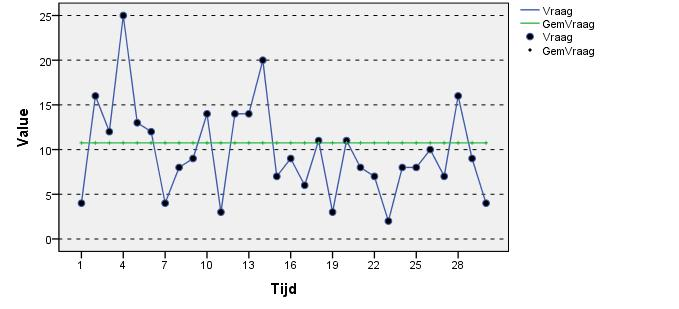
\includegraphics[width=1.00\textwidth]{images/tijdsreeksen/tijdsreeks21.jpg}
%	\caption{Tijdreeks met constant gemiddelde}
%	\label{fig:tijdreeks21}
%\end{figure}
%
%
%Indien we veronderstellen dat de data verandert met de tijd is het beter om oude data minder waarde te geven en de recente data meer waarde. Een mogelijkheid is om enkel recente data te gebruiken, bijvoorbeeld de 10 (zie fig. \ref{fig:tijdreeks31}) en 5 laatste datapunten (zie figuur \ref{fig:tijdreeks41}).
%
%\[ \widehat{b} = \frac{1}{10} \sum_{10}^{20} x_{t} = 10.18 \] en
%\[ \widehat{b} = \frac{1}{5} \sum_{15}^{20} x_{t} = 7.83 \]
%
%\begin{figure}
%	\centering
%		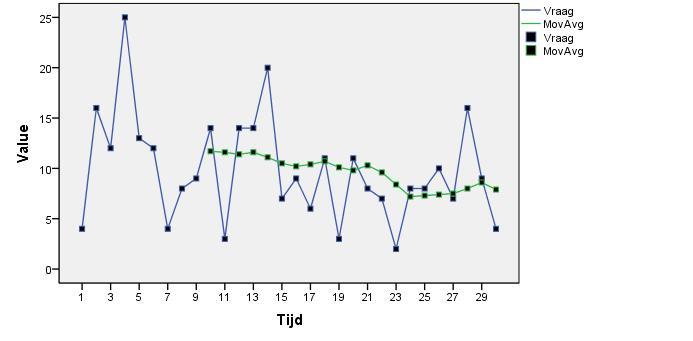
\includegraphics[width=1.00\textwidth]{images/tijdsreeksen/tijdsreeks31.jpg}
%		\caption{Tijdreeks met moving average $m = 10$}. 
%	\label{fig:tijdreeks31}
%\end{figure}
%
%\begin{figure}
%	\centering
%		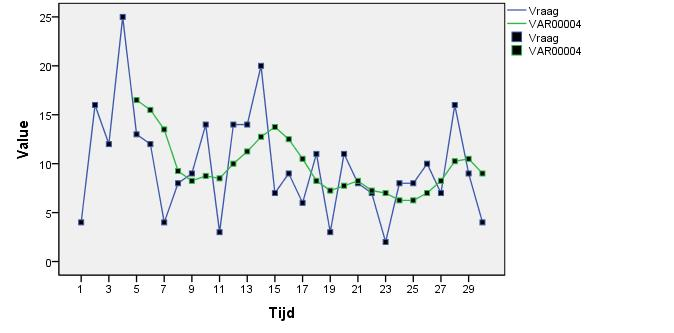
\includegraphics[width=1.00\textwidth]{images/tijdsreeksen/tijdsreeks41.jpg}
%	\caption{Tijdreeks met moving average $m = 5$}
%	\label{fig:tijdreeks41}
%\end{figure}
%
%
%
%Dit worden \textit{moving averages} genoemd \index{moving average}. 
%
%Welke schatter is nu de beste? We kunnen dit nu nog niet zeggen. 
%\begin{itemize}
%	\item De schatter die alle datapunten gebruikt is de beste indien de tijdreeks het model volledig volgt.
%	\item De schatter met de recentere datapunten is de beste indien de tijdreeks verandert met de tijd.
%\end{itemize}
%
%\begin{definition}
%	Algemeen is het moving average het gemiddelde van de $m$ laatste observaties.
%	\begin{equation}
%		\widehat{b} = \sum_{i=k}^{t} \frac{x_{i}}{m}
%	\label{eq:movingAverage}
%	\end{equation}
%	met $k = t-m+1$. $m$ is de time range en is de parameter van de methode.
%\end{definition}
%
%
%\begin{table}
%    \begin{tabular}{|lllllllllll|}
%    \hline
%    ~         & 11   & 12   & 13   & 14   & 15   & 16   & 17   & 18   & 19   & 20   \\
%    Data      & 3    & 14   & 14   & 20   & 7    & 9    & 6    & 11   & 3    & 11   \\
%    Schatting & 11.7 & 11.6 & 11.4 & 11.6 & 11.1 & 10.5 & 10.2 & 10.4 & 10.7 & 10.1 \\
%    Error     & -8.7 & 2.4  & 2.6  & 8.4  & -4.1 & -1.5 & -4.2 & 0.6  & -7.7 & 0.9  \\ \hline
%    \end{tabular}
%		\caption{Voorspellingsfout voor een moving average $m = 10$}
%		\label{tab:error}
%\end{table}
%
%\subsection{Meten van de nauwkeurigheid van voorspellingen}
%
%Een methode om de voorspelling te meten is het gemiddelde van de deviaties ($MAD$): gemiddelde absolute verschil tussen het voorspelde en de werkelijke waarden van de tijdsreeks.
%
%\begin{definition}[$MAD$]
%\begin{equation}
%	MAD = \frac{1}{n} \sum_{1}^{n} \left| e_{i} \right|  
%\label{eq:MAD}
%\end{equation}
%\end{definition}
%
%Je kan dit ook percenteren om zo tot de gemiddelde absolute procentuele afwijking ($MAPE$) te komen.
%
%\begin{definition}[$MAPE$]
%\begin{equation}
%	MAPE = \frac{1}{n} \sum_{1}^{n} \left| \frac{e_{i}}{X_i} \right|  
%\label{eq:MAD2}
%\end{equation}
%\end{definition}
%
%
%Je kan ook de variantie ervan bepalen:
%
%\begin{definition}[$VAR$]
%\begin{equation}
%	s^{2}_{e} = \frac{1}{m} \sum_{1}^{n} (e_{i} - \overline{e})^{2}
%\label{eq:varError}
%\end{equation}
%\end{definition}
%
%Als laatste interessante parameter kan gekeken worden naar de wortel uit de gemiddelde kwadratische afwijking ($RMSE$), als de wortel uit het gemiddelde kwadratische verschil tussen de voorspelde en de werkelijke waarden van de tijdsreeks.
%
%\begin{definition}[$RMSE$]
%\begin{equation}
%	RMSE_{e} = \sqrt{\frac{1}{m} \sum_{1}^{n} (e_{i})^{2}}
%\label{eq:varError2}
%\end{equation}
%\end{definition}
%
%
%\section{Exponenti\"ele smoothing}
%Bij een moving average krijgen alle voorgaande observaties een gelijk gewicht. Bij exponentieel smoothing worden kleinere gewichten toegekend aan oudere observaties. M.a.w.: recente observaties krijgen relatief meer gewicht dan oudere observaties.
%
%In het geval van moving average zijn de gewichten hetzelfde, namelijk $\frac{1}{m}$.
%
%\subsection{Enkelvoudige exponenti\"ele smoothing}
%Exponenti\"ele effening (of smoothing) is een gewogen gemiddlede dat positieve gewichten toekent aan de huidige waarden en waarden uit het verleden van de tijdsreeks. Een enkel gewicht, $0\leq \alpha \leq1$ of de exponentie\"ele effeningsconstante wordt hiervoor gekozen. 
%Voor een tijdseenheid $T$ wordt het enkelvoudige exponenti\"ele smoothing gevonden door vergelijking \ref{eq:singleExpSmooting}.
%
%\begin{definition}[Exponenti\"ele smoothing]
%\begin{equation}
%	X_{T} = \alpha x_{t-1} + (1-\alpha)X_{t-1}, 0 \leq \alpha \leq 1, t \geq 3
%\label{eq:singleExpSmooting}
%\end{equation}
%\end{definition}
%
%$\alpha$ wordt de smoothing constante genoemd.
%
%\subsubsection{Inti\"ele setting}
%Het bepalen van $X_{2}$ is een belangrijke parameter. Men kan kiezen om:
%\begin{enumerate}
%	\item $X_{2} = x_{1}$ te stellen
%	\item $X_{2}$ gelijk te stellen aan een bepaald objectief
%	\item Een gemiddelde te nemen van de eerste $x$ observaties
%	\item \dots
%\end{enumerate}
%
%\begin{exercise}
%	Waarom wordt dit een exponenti\"ele methode genoemd?
%\end{exercise}
%Antwoord: als we zouden substitueren vinden we bv. voor $X_{t-1}$:
%
%\[ X_{t} = \alpha x_{t-1} + (1-\alpha)\left[\alpha x_{t-2} + (1-\alpha)X_{t-2}\right] \] 
%\[ X_{t} = \alpha x_{t-1} + \alpha (1-\alpha)x_{t-2} + (1-\alpha)^{2} X_{t-2} \]
%of dus algemeen gesteld :
%\[ X_{t} = \alpha \sum_{i=1}^{t-2}(1-\alpha)^{i-1}x_{t-i} + (1-\alpha)^{t-2} X_{2}, t \geq 2 \]
%
%Zo merk je dat oudere componenten een exponentieel kleiner gewicht verkrijgen. 
%
%\subsubsection{Waarde voor $\alpha$}
%De snelheid waarmee de oude observaties ''vergeten`` worden hang af van $\alpha$. Met een $\alpha$ dicht bij 1 vergeet je snel, terwijl een $\alpha$ dicht bij nul ervoor zorgt dat vergeten minder snel gaat (zoals aangetoond in tabel \ref{tab:alpha}). Vaak wordt een waarde gebruikt tussen $0.10$ en $0.30$.
%
%\begin{table}
%\centering
%    \begin{tabular}{l|llll}
%    $\alpha$ & $(1-\alpha)$ & $(1-\alpha)^{2}$ & $(1-\alpha)^{3}$ & $(1-\alpha)^{4}$ \\ \hline
%    0.9   & 0.1       & 0.01             & 0.001                      & 0.0001           \\
%    0.5   & 0.5       & 0.25             & 0.125                      & 0.062            \\
%    0.1   & 0.9       & 0.81             & 0.729                      & 0.6561           \\
%    \end{tabular}
%		\caption{Waarden voor $\alpha$ en $(1-\alpha)^{n}$}
%		\label{tab:alpha}
%\end{table}
% 
%In figuur \ref{fig:tijdreeks51} vind je de tijdreeksen voor $\alpha=0.1 , 0.5, 0.9$.  
%
%\begin{figure}[htbp]
%	\centering
%		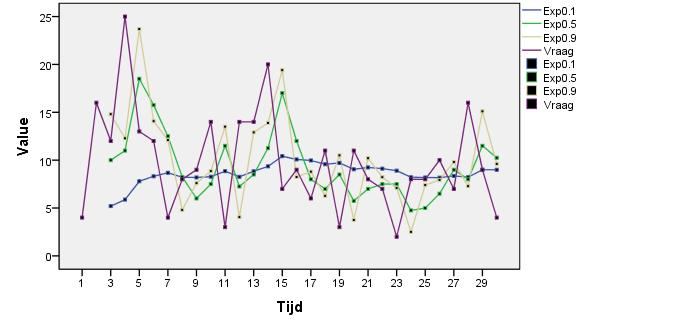
\includegraphics[width=1.00\textwidth]{images/tijdsreeksen/tijdsreeks51.jpg}
%	\caption{Enkelvoudig exponentieel model voor $\alpha=0.1 , 0.5, 0.9$}
%	\label{fig:tijdreeks51}
%\end{figure}
%
%\subsubsection{Voorspelling met exponenti\"ele effening}
%Stel dat het doel is om de volgende waarde $X_{t+1}$ te voorspellen, dan wordt dit gelijk gesteld aan de smoothing waarde op tijdstip $t$.
%
%\begin{equation}
%	X_{t+1} = EMA_t = X_t + \alpha(x_t - X_t)
%	\label{eq:EMA}
%\end{equation}
%
%\subsection{Dubbele exponenti\"ele smoothing}
%Enkelvoudige smoothing wordt gebruikt wanneer er geen trend zichtbaar is. Wanneer er een trend (stijgend of dalend) is dan kan er iets fout gaan. Zie bijvoorbeeld de data in tabel \ref{tab:trend} en figuur \ref{fig:tijdreeks61}.
%
%\begin{table}
%\centering
%    \begin{tabular}{|ll|}
%    \hline
%    Data & Enkelvoudige smoothing \\
%    6.4  & ~                      \\
%    5.6  & 6.4                    \\
%    7.8  & 6.2                    \\
%    8.8  & 6.7                    \\
%    11.0 & 7.3                    \\
%    11.6 & 8.4                    \\
%    16.7 & 9.4                    \\
%    15.3 & 11.6                   \\
%    21.6 & 12.7                   \\
%    22.4 & 15.4                   \\ \hline
%    \end{tabular}
%		\caption{Enkelvoudige smoothing met $\alpha = 0.3$}
%		\label{tab:trend}
%\end{table}
%
%\begin{figure}
%	\centering
%		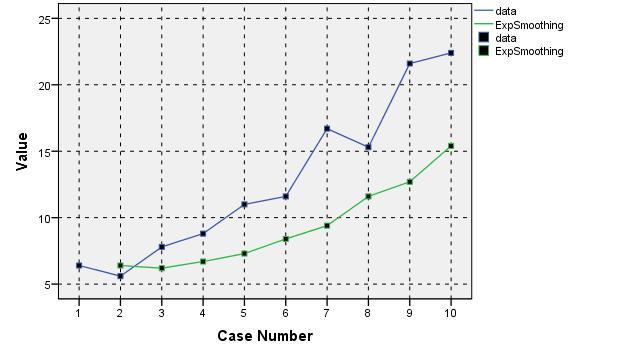
\includegraphics[width=1.00\textwidth]{images/tijdsreeksen/tijdsreeks61.jpg}
%	\caption{Exponenti\"ele smoothing bij een trend}
%	\label{fig:tijdreeks61}
%\end{figure}
%
%Daarom voegen we een extra constante toe om deze trap te overbruggen:
%
%\begin{definition}[Holt-voorspelling of dubbele exponenti\"ele voorspelling]
%\begin{eqnarray}
%	X_{t} = \alpha x_{t} + (1-\alpha)(X_{t-1} + b_{t-1}) & 0 \leq \alpha \leq 1 \\
%	b_{t} = \gamma(X_{t}-X_{t-1}) + (1-\gamma)b_{t-1} & 0 \leq \gamma \leq 1 
%\label{eq:doubleSmoothing}
%\end{eqnarray}
%\end{definition}
%
%\subsubsection{Initi\"ele waarde}
%Net zoals in enkelvoudige smoothing kan je verschillende methodes kiezen om initi\"ele waardes voor $X_{t}$ en $b_{t}$ te kiezen:
%\begin{itemize}
%	\item $X_{1} = x_{1}$
%	\item $b_{1} = x_{2} - x_{1}$
%	\item $b_{1} = \frac{1}{3}\left[ (x_{2} - x_{1}) + (x_{1} - x_{2}) + (x_{4} - x_{3}) \right]$
%	\item $b_{1} = \frac{x_{n} - x_{1}}{n-1}$
%\end{itemize}
%
%\subsubsection{Voorspelling}
%Een voorspelling maken met dubbele exponenti\"ele smoothing gebeurt dan iets anders (noem $F_{t+1}$ de voorspelling voor tijd $T+1$):
%
%\[ F_{t+1} = X_{t} + b_{t} \]
%of
%\[ F_{t+m} = X_{t} + m b_{t} \]
%
%Als we nu de tekening maken met enkelvoudige smoothing ($\alpha = 0.977$) en dubbele smoothing ($\alpha = 0.3623, \gamma = 1.0, X_{1} = x_{1} = 6.4$ en $b_{1} = \frac{1}{3}\left[ (x_{2} - x_{1}) + (x_{1} - x_{2}) + (x_{4} - x_{3}) \right] = 0.8$ vinden we volgende waarden in tabel \ref{tab:doubleSingle} en figuur \ref{fig:tijdreeks71}:
%
%\begin{table}
%\centering
%    \begin{tabular}{|llll|}
%    \hline
%    Data & Enkelvoudige smoothing $X_{t}$ & Double smoothing $X_{t}$ & $F_{t}$ \\
%    6.4  & ~                      & 6.4              & ~                             \\
%    5.6  & 6.4                    & 6.6              & 7.2                           \\
%    7.8  & 5.6                    & 7.2              & 6.8                           \\
%    8.8  & 6.7                    & 8.1              & 7.8                           \\
%    11.0 & 8.8                    & 9.8              & 9.1                           \\
%    11.6 & 10.9                   & 11.5             & 11.4                          \\
%    16.7 & 11.6                   & 14.5             & 13.2                          \\
%    15.3 & 16.6                   & 16.7             & 17.4                          \\
%    21.6 & 15.3                   & 19.9             & 18.9                          \\
%    22.4 & 21.5                   & 22.8             & 23.1                          \\ \hline
%    \end{tabular}
%		\caption{Tabel met enkelvoudige en dubbele smoothing}
%		\label{tab:doubleSingle}
%\end{table}
%
%\begin{figure}
%	\centering
%		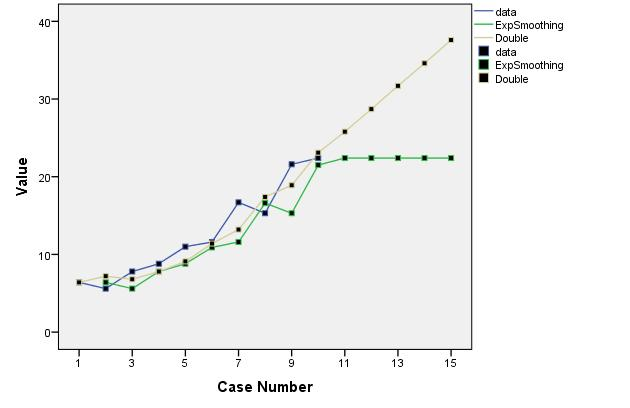
\includegraphics[width=1.00\textwidth]{images/tijdsreeksen/tijdsreeks71.jpg}
%	\caption{Enkelvoudige en dubbele smoothing}
%	\label{fig:tijdreeks71}
%\end{figure}
%
%\subsection{Driedubbele exponenti\"ele smoothing}
%Wanneer dubbele smoothing niet werkt kan driedubbele smoothing gebruikt worden, ofwel Holt-Winters methode genoemd.
%
%\begin{eqnarray}
%	X_{t} = \alpha \frac{x_{t}}{c_{t-L}} + (1-\alpha) (X_{t-1} + b_{t-1}) & \textnormal{Smoothing}\\
%	b_{t} = \gamma (X_{t} - X_{t-1}) + (1-\gamma)b_{t-1} & \textnormal{Trend smoothing} \\
%	c_{t} = \beta \frac{x_{t}}{X_{t}} + (1-\beta)c_{t-L} & \textnormal{Seasonal smoothing} \\
%	F_{t+m} = (X_{t} + mb_{t})c_{t-L+m} & \textnormal{Voorspelling}
%\label{eq:HoltWinters}
%\end{eqnarray}
% met 
%\begin{itemize}
%	\item $x_{t}$ de observatie op tijdstip $t$
%	\item $X_{t}$ is de smoothed observatie op tijdstip $t$
%	\item $b_{t}$ is de trendfactor op tijdstip $t$
%	\item $c_{t}$ is de seizoensindex op tijdstip $t$
%	\item $F_{t}$ is de voorspelling op tijdstip $t$
%	\item $L$ is de periode (bv. van de seizoenen)
%\end{itemize}
%
%$\alpha, \beta, \gamma$ zijn constanten die geschat moeten worden. 
